% Chapter Template

\chapter{Clean Architecture} % Main chapter title

\label{Chapter5} % Change X to a consecutive number; for referencing this chapter elsewhere, use \ref{ChapterX}

\lhead{Capítulo  5. \emph{Clean Architecture}} % Change X to a consecutive number; this is for the header on each page - perhaps a shortened title

%----------------------------------------------------------------------------------------
%	SECTION 1
%----------------------------------------------------------------------------------------

\section{Modelos de Implementación Clean Architecture}

Los mejores intentos de implementación de esta arquitectura vienen de la mano de un colega Fernando Cejas y el ejemplo de los Blueprints de Google.

\begin{figure}[htbp]
	\centering
	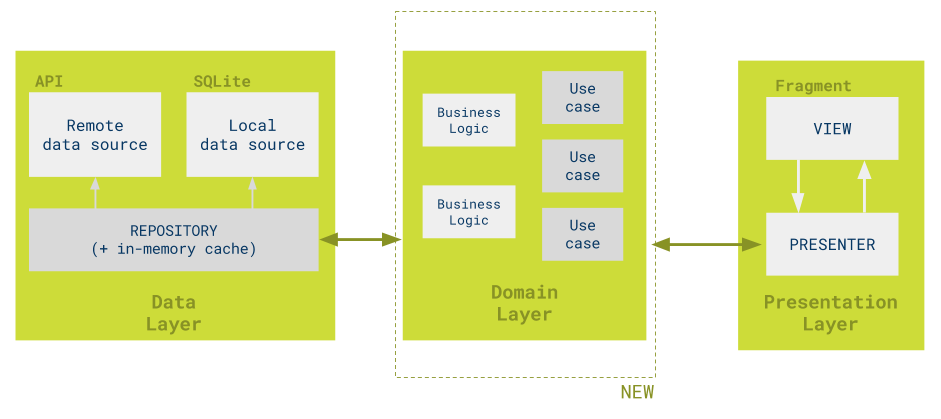
\includegraphics[width=1\textwidth]{Figures/-006.png}
	\rule{35em}{1pt}
	\caption[Principio de Dependecias]{Esquema de dependencias para una arquitectura en capas.}
	\label{fig:Diagrama_clasico}
\end{figure}

Ambas implementaciones están compuestas de tres capas distintas:

\begin{itemize}
	\item Presentation Layer: Esta capa se encarga de interactuar con la UI. Implementa un patrón de diseño conocido como \textbf{MVP (Model View Controller)}. 
	\item Domain Layer: Esta capa contiene toda la lógica de negocio. La capa de dominio comienza con las clases denominadas casos de uso o interactores según la literatura, utilizados por los presentadores de la aplicación. Estos casos de uso representan todas las acciones posibles que un desarrollador puede realizar desde la capa de presentación. Los casos de uso se implementaron utilizando el patrón de diseño conocido como \textbf{Commander}.
	\item Data Layer: Esta capa administra la adquisición de datos y es capaz de utilizar diferentes fuentes de datos. Esta capa se suele implementar utilizando el patrón de diseño conocido como \textbf{Repository}.  
\end{itemize}

